\documentclass[palatino,nosec]{Docencia}


\title{Cuaderno de clase}
\author{Víctor de Juan}
\date{20/21}

\begin{abstract}
%Cuaderno de clase de Matemáticas I, con el desarrollo continuado (sin estar separado por sesiones).
Desarrollo del inicio de la geometría analícita bidimensional, temario de Matemáticas I.
\end{abstract}



% Paquetes adicionales

\usepackage[author={Departamento Matemáticas, 2019}]{pdfcomment}
\newcommand{\kinz}{,\;k\in\mathbb{Z}}

\makeatletter
\newcommand{\annotate}[2][]{%
\pdfstringdef\x@title{#1}%
\edef\r{\string\r}%
\pdfstringdef\x@contents{#2}%
\pdfannot
width 2\p
height 2\baselineskip
depth 0pt
{
/Subtype /Text
/T (\x@title)
/Contents (\x@contents)
}%
}
\makeatother

% --------------------
\newcommand{\cimplies}{\text{\hl{$\implies$}}}
\renewcommand{\vx}{\overset{\rightarrow}{x}}
\renewcommand{\vy}{\overset{\rightarrow}{y}}
\renewcommand{\vz}{\overset{\rightarrow}{z}}
\newcommand{\vi}{\overset{\rightarrow}{i}}
\newcommand{\vj}{\overset{\rightarrow}{j}}
\renewcommand{\vec}[1]{\overset{\rightarrow}{#1}}

\usepackage{pgf,tikz}
\usetikzlibrary{arrows}

\begin{document}
\pagestyle{plain}
\maketitle
\tableofcontents


%% Contenido.

% \chapter{Primera evaluación}

% \section{Introducción a la asignatura}

% \hl{Sed “críticos” en general}. Lo que os cuenten razonadlo. No os lo creáis sin más. Y de esto, nos vamos a hartar en Matemáticas.

% \subsubsection{Temario de la asignatura}

% El \hl{orden} que vamos a seguir difiere un poco del del libro, porque así nos parece a MariNieves y a mi. 

% Teoría de números: 

% Vamos a dar uno de los temas más bonitos de todo el bachillerato. ¡\hl{Los números complejos}! ¿A alguien le dice algo? ¿A alguien le suena? 
% %
% Ya veréis que, en realidad, no son difíciles. Simplemente arrastramos $\sqrt{-1}$ en las operaciones, como una expresión algebraica, llamando $i=\sqrt{-1}$. 
% %
% Precioso. 

% Vamos a dar un paso más en la resolución de \hl{ecuaciones y sistemas}. 
% %
% El año pasado resolvíais ecuaciones del tipo: $81^{2x} = \frac{1}{3};\quad x-\sqrt{x-3} = \sqrt{x-2}$, sistemas de ecuaciones 2x2... Este año vamos a ir más allá, vamos a resolver sistemas de 3x3. 

% El año pasado tuvisteis una introducción a la geometría. Este año vamos a trabajar con \hl{problemas serios el plano}: distancia punto a recta, distancia entre rectas, cónicas... Por cierto, \ul{¿sabéis porqué se llaman cónicas?}

% Y ahora que ya sabéis algo de trigonometría, vamos a ir más allá. Vamos a \hl{exprimir la trigonometría} hasta dominarla. Es algo fundamental en matemáticas. 



% Y uno de los contenidos centrales del curso, del que hablaréis cuando terminéis el colegio y habréis oído hablar... Las míticas \hl{derivadas}. Os suena, ¿no? 
% %
% Pues este año nos meteremos en ese berenjenal, a aprender qué es una derivada y para que sirve.
% %
% También veremos las \hl{Integrales}.
% %
% Terminaremos el curso con probabilidad y estadística.

% Todo esto es una visión general del temario del curso. 
% %
% Pero hay otro aspecto fundamental de la asignatura. 
% %
% En otros años lo fundamental puede ser coger habilidad y soltura en los cálculos, saber resolver los problemas... 
% %
% Este curso va de \hl{razonar y justificar}. Me importa relativamente poco si el resultado está bien o no, en comparación con lo que me importa si el procedimiento está razonado y justificado. 
% %
% Las matemáticas no son magia, todo tiene una razón de ser. Todo tiene una explicación. 
% %
% Por ejemplo, ya no nos vamos a centrar tanto en "resuelve esto o lo otro", sino en "demuestra, comprueba, discute esto o lo otro".
% %
% ¿Se entiende?

% Por ejemplo, ¿porqué el \hl{teorema de Pitágoras} funciona? 
% %
% Claro, porque probando con unos números funciona. 
% %
% ¿Quién te asegura que para absolutamente cualquier triángulo rectángulo va a funcionar? Eso hace 4 años te lo creíste. 
% %
% Este año vamos a demostrar el teorema.

% En general, va a haber pocos actos de fe. 
% %
% En el curso habrá demostraciones y los contenidos no vendrán dados por arte de magia. 
% %
% Ojo, el teorema fundamental del álgebra no lo podremos demostrar porque hacen falta matemáticas más complejas. 
% %
% Todo lo demás, lo podremos demostrar.

% \subsection{Metodología de clase}

% \subsection{Criterios de evaluación}


% \begin{itemize}
% 	\item 10\%: llevarlo al día.
% 	    \subitem 10\%, 30\%, 60\%. Estudiar al día. Tutorías a demanda. Cosas que tenéis que saber, aunque, seminarios.

%     	\subitem Pruebecita del lunes, tal vez con teoría.

% 	\item 30\%: primer parcial.
% 	\item 60\%: segundo parcial.
% \end{itemize}



%
\chapter{Números y complejos}

\subsubsection{Conjuntos numéricos}

¿Qué conjuntos de números conocéis? $ℕ,ℤ,ℚ,I,ℝ,ℂ$ \hl{Diagrama de contenidos} e historia de cómo van surgiendo.

\textit{Si sobrara tiempo: belleza intrínseca de las matemáticas: ¿Qué hay más, enteros o pares?}

%10 minutos

Cómo distinguir que un número dado pertenece a un conjunto o no.
%
Por ejemplo, $\sqrt{2}$. ¿A qué conjunto pertenece y porqué?
%
\hl{¿Por qué $\sqrt{2}$ es irracional?} $\rfrac{4}{3} = 1.\hat{3}$ también tiene infinitos decimales.
%
En este curso ya no vale creerse lo que los profesores os contamos sin más. Es fundamental entender las demostraciones y ser capaz de razonar el porqué de los asuntos.


\begin{proof}[\textbf{Reducción al absurdo}]
Suponemos $\sqrt{2}\in ℚ$.

Entonces 
\[
	\exists a,b\inℤ \tq \left(\sqrt{2} = \rfrac{a}{b}\right) \wedge \left( \mcd{a,b} = 1 \right)
\]


\[
	\sqrt{2} = \frac{a}{b} \implies 2·b^2 = a^2 \implies a^2 \text{ es par} \overset{1}{\implies} a \text{ es par}
\]

Si $a^2$ es par, necesariamente $a$ es par también. Por reducción al absurdo, si $a$ no fuera par, $a·a$, producto de impares no sería par. 
%
Como $a$ es par, podemos escribirlo como $a=2·k$, para algún $k\in ℤ$. 

\[
	2b^2 = (2k)^2 \implies b^2 = 2k^2 \overset{1}{\implies} b \text{ par}.
\]

Conclusión: $\mcd{a,b} = 2 ≠ 1$. Hemos llegado a una contradicción partiendo de un supuesto ($\sqrt{2}\in ℚ$) "inventado", por lo que ese supuesto debe ser falso. 

\paragraph{Un argumento alternativo} no tan convincente aunque más fácil de entender sería: 

$2·b^2 = a^2$. Así, en la descomposición factorial de $a^2$ aparecería el factor $b^2$, por lo que $\mcd{a^2,b^2}=b^2$.

\[
\left.
\begin{array}{c}
	\mcd{a,b} = 1 \implies \mcd{a^2,b^2} = 1\\
	\mcd{a^2,b^2}=b^2
\end{array}\right\} \implies b=\pm 1 \implies \sqrt{2}\in ℤ
\]

\end{proof}

%Hasta los 40 minutos

\paragraph{\hl{No os creáis cualquier demostración:}}
Partiendo de $x=y$

\[
x^2 = xy \dimplies x^2-y^2 = xy-y^2 \dimplies (x+y)(x-y) = y(x-y) \dimplies x+y = y \dimplies 2y = y \implies \text{\hl{2=1}}
\]




\section{Introducción} 
Vamos a interntar resolver $x^2 + 9 = 0 \dimplies x^2 = -9 \dimplies x=\sqrt{-9}$. Siempre hemos dicho que no tiene solución. Pero yo podría escribir $(\sqrt{-9})^2 + 9 = 0$. Es decir, $\sqrt{-9}$ es solución de la ecuación. ¡Y también lo es $x_2=-\sqrt{-9}$!

La manera de trabajar con raíces negativas es sacar todos los factores hasta dejar simplemente $\sqrt{-1}$, es decir: $\sqrt{-9} = \sqrt{9}\sqrt{-1} = \pm3\sqrt{-1}$ y escribimos $\sqrt{-1} = i$. \textbf{Conclusión:} las soluciones de la ecuación son $x_1 = 3i$ y $x_2 = -3i$.

Podemos resolver ecuaciones que antes eran imposibles y, además, podemos calcular raíces que antes no "existirían".

%(Hasta aquí la introducción)

Pongamos otro ejemplo:


¿Podríamos factorizar el polinomio $P(x) = x^2-2x+2$? El \textbf{teorema fundamental del álgebra} dice que tiene 2 soluciones, pero las 2 son complejas. Vamos a verlo

Para factorizar el polinomio calculamos sus raíces resolviendo la ecuación: $P(x) = 0$

\[x^2-2x+2 = 0 \dimplies x=\frac{2\pm\sqrt{4-4·1·2}}{2} = \frac{2\pm\sqrt{-4}}{2} = \frac{2}{2} \pm \frac{2i}{2} = 1\pm i\]

Hemos obtenido 2 raíces: $α_1 = 1+i$ y $α_2 = 1-i$. ¿Cómo quedaría el polinomio factorizado? \[P(x) = x^2-2x+2 = (x-α_1)·(x-α_2) = (x-(1+i))·(x-(1-i))\]

Primera utilidad de los números complejos: resolver ecuaciones que antes eran "imposibles" y factorizar polinomios que considerábamos irreducibles.

Hay otra utilidad más: $\sqrt[6]{64}$ tiene 6 soluciones: $\sqrt[6]{64} = \{ 2,-2,1+\sqrt{3},1-\sqrt{3},-1+\sqrt{3},-1-\sqrt{3}\}$. ¿Las comprobamos entre todos?

\section{Formalización y operaciones en $ℂ$}

Un número complejo es de la forma $z=a+bi$, donde $i=\sqrt{-1}$, y llamamos $a=Re(z)$ y $b=Im(z)$. 

\paragraph{Ejemplos}
\begin{itemize}
	\item $z_1 = 3$ $\to$ $Re(z_1) = \;\;\quad\quad\;\;\;$; $Im(z_1) = \;\;\;\;\;\;\;$ \footnote{Luego, todos los números reales son complejos.}
	\item $z_2 = 2-i$ $\to$ $Re(z_2) = \;\;\quad\quad\;\;\;$; $Im(z_2) = \;\;\;\;\;\;\;$
	\item $z_3 = \sqrt{2}+6i$ $\to$ $Re(z_3) = \;\;\quad\quad\;\;\;$; $Im(z_3) = \;\;\;\;\;\;\;$
\end{itemize}



\paragraph{Representación gráfica:} como los vectores en física, sólo que aquí no hay $\vec{i}$ ni $\vec{j}$. El eje $y$ es el eje \textit{imaginario} y el eje $x$ es el eje \textit{real}.

\begin{example} Representa los números complejos $z_1 = 1-i;\;z_2 = 0;\; z_3 = 2+3i$.

\begin{figure}[hbtp]
\centering
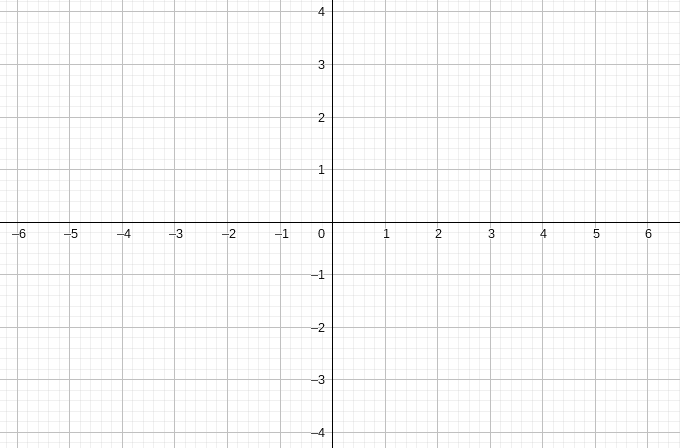
\includegraphics[scale=0.5]{../grid.png}
\end{figure}
\end{example}

\begin{defn}[Complejos\IS Conjugado] Llamamos conjugado de un número complejo $z = a+bi$ a $\bar{z} = a-bi$.

\obs Los conjugados son simétricos respecto del eje $x$.
\end{defn}

\subsection{Operaciones en forma binómica} 

\[
[(2+i)+(3-2i) - (-2i)]·[(\rfrac{1}{5}+i)] = ...
\]

\paragraph{División}

Para dividir $z_1 = a+bi$ entre $z_2 = c+di$ hacemos:

\[
\frac{z_1}{z_2} = \frac{a+bi}{c+di} = \frac{a+bi}{c+di} \frac{c-di}{c-di} = \frac{z_1}{z_2}·\frac{\bar{z_2}}{\bar{z_2}}
\]

¿Por qué se multiplica por el conjugado? En la división buscamos $z_? = x+yi$ tal que:

\[\frac{z_1}{z_2} = \frac{a+bi}{c+di} = x+yi\]

Al multiplicar arriba y abajo por el conjugado estamos quitando el número complejo del denominador. De esa manera, operando podemos obtener $x$ e $y$.


\textbf{Ejemplo: }


\paragraph{Practicar con el ejercicio 8} 

\subsubsection{Forma polar}


\begin{example}
 $z = 1-i$, dibujando el punto y sacando el ángulo que forma. 

$|z| = \sqrt{1^2+1^2} = \sqrt{2}$

$\alpha_z = \frac{-\pi}{4}$

$z = 1-i = \sqrt{2}_{\rfrac{-\pi}{4}}$

\end{example}

En la representación gráfica de números complejos, podemos utilizar otro sistema de referencia: \textit{módulo} $|z|=r$ y \textit{argumento (ángulo)} $\arg{z} = α$. 
%
Estas son las \concept[Coordenadas polares complejos]{coordenadas polares} de un número complejo y escribimos $z = r_α$


Sea $z=a+bi \in\mathbb{C}$, definimos \concept[Complejos\IS Módulo]{módulo} como $|z| = +\sqrt{a^2+b^2}$.

\obs La representación geométrica del módulo es la distancia hasta el origen de coordenadas.

Sea $z=a+bi \in\mathbb{C}$, definimos \concept[Complejos\IS Argumento]{argumento} como $\alpha = \arctg\left(\frac{Im(z)}{Re(z)}\right)$.


\textbf{Escribe en forma polar:}
\begin{itemize}
	\item $z_1 = 1+i$
	\item $z_2 = 1-i$
	\item $z_3 = 6i$
	\item $z_4 = -2-\sqrt{3}i$
\end{itemize}

\paragraph{Transformación de forma polar a binómica} Dado $z = r_α$, las coordenadas en el plano del número complejo son $(r\cos(α),r\sin(α))$, por lo que podemos escribir:

\[z = \underbrace{r_{α}}_{\text{Polar}} = \underbrace{r·(\cos(α) + i\sin(α))}_{\text{Trigonométrica}} = \underbrace{r\cos(α)}_{a}+\underbrace{r\sin(α)}_{b}i = \underbrace{a+bi}_{\text{Binómica}}\]

\paragraph{Operaciones en forma polar y trigonométrica}

Sean $z_1 = r_α$ y $z_2 = s_β$

$z_1\pm z_2$ necesitamos pasar a forma binómica/trigonométrica. ¿Para qué sirve esta forma entonces? Para multiplicar y dividir, que se hace realmente sencillo 

\hl{Corregir 8ef, 15 abc (solo polar)}. Introducir trigonométrica desde el ejercicio 15.

Operaciones en polar.

\textbf{Multiplicación:} $z_1·z_2 = (r·s)_{α+β} $

Ver \ref{trigon:multicomplejapolar} para la demostración.

\textbf{División:} $\frac{z_1}{z_2} = (\rfrac{r}{s})_{α-β} $

\textbf{Ejemplo}
\[\frac{3_{30}·5_{120}}{\sqrt{15}_{60}·1_{420}}\]


\[\frac{2_{120}·1_{240}}{\sqrt{2}_{60}·2_{30}}\]


\section{Radicación}

Sabemos que $\sqrt{16} = \pm 4$, ¿verdad? Y $\sqrt[4]{16} = \pm 2$, ¿no?

¿Nos habrán mentido desde pequeños sobre esto también? Siento decirte que sí. Vamos a verlo. 

Calcula:
\begin{itemize}
	\item $2^4 = 16$
	\item $(-2)^4 = 16$
	\item $(2i)^4 = 16·i^4 = 16$
	\item $(-2i)^4 = 16·i^4 = 16$ 
\end{itemize}

¡Cuatro raíces! De una manera general $\sqrt[n]{z}$ tiene $n$ soluciones. ¡Vamos a calcularlas! Y para esto es imprescindible la forma polar.

\begin{defn}[Radicación compleja]
$\sqrt[n]{z} = \{s_β\}$ con $s=+\sqrt[n]{|z|}$ y $β=\left\{\displaystyle\frac{\arg(z)+360k}{n}\;\;k\inℕ\right\}$
\end{defn}

\begin{example}
Calcula las 5 raíces de $z=1+i$

\textbf{Solución}
\begin{itemize}
	\item Forma polar: $z=1+i = \sqrt{2}_{45}$
	\item Las raíces serán de la forma $s_β$ con $s=\sqrt[5]{\sqrt{2}}$ y $β=\frac{45+360k}{5}$
	\begin{itemize}
		\item $k=0\to \sqrt[10]{2}_{9}$
		\item $k=1\to \sqrt[10]{2}_{81}$
		\item $k=2\to \sqrt[10]{2}_{153}$
		\item $k=3\to \sqrt[10]{2}_{225}$
		\item $k=4\to \sqrt[10]{2}_{297}$
	\end{itemize}
\end{itemize}
\end{example}



%% -*- root: ../Cuaderno.tex -*-

\chapter{Álgebra}

\section{Repaso de 4º}

\subsection{Logaritmos}

\paragraph{Introducción}

Vamos a aprender una nueva manera de multiplicar. En realidad ya sabéis, aunque no seáis conscientes.\footnote{Fuente: \href{https://www.youtube.com/watch?v=FB3\_BeukBBk\&t=99s}{Mark Foskey, youtube.com}}


\begin{itemize}
\item Caso 1: $1000000·10000000 = 10^6·10^7 = 10^{13}$. ¿Y podremos hacer esto con otros números que no sean el 10?

\item Caso 2: $64·128 = 2^6·2^7 = 2^{13} = 8192$
\item ¿Caso 3?: Me construyo la tabla del 3.
\begin{center}
\begin{tabular}{cccccccccccc}
1& 3& 9& 27& 81& 243& 729& 2187& 6561& 19683& 59049& 177147\\
\textcolor{red}{0} & \textcolor{red}{1} & \textcolor{red}{2} & \textcolor{red}{3} & \textcolor{red}{4} & \textcolor{red}{5} & \textcolor{red}{6} & \textcolor{red}{7} & \textcolor{red}{8} & \textcolor{red}{9} & \textcolor{red}{10} & \textcolor{red}{11}
\end{tabular}
\end{center}
\item Caso 4: ¿Y para números que no son potencias enteras? Por ejemplo, $64*40$. Pues si $32=2^5$ y $64=2^6$, $40=2^{5,...}$ ¿Tiene sentido?

\item Caso 5: Lo que hicieron, Yost y Napier, fue coger la tabla del 1,0001 en lugar de la tabla del 3 y dividir por mil los números rojos, dando lugar a la tabla de logaritmos:

\begin{center}
	\begin{tabular}{cl}
		0.0 & 1.0\\
		0.001 & 1.001\\
		0.002 & 1.002\\
		0.003 & 1.003\\
		0.004 & 1.00401\\
		0.005 & 1.00501\\
		0.006 & 1.00602\\
		0.007 & 1.00702\\
		0.008 & 1.00803\\
		0.009 & 1.00904\\
		$\vdots$ & \quad\quad$\vdots$\\
		0.991 & 2.69259\\
		0.992 & 2.69529\\
		0.993 & 2.69798\\
		0.994 & 2.70068\\
		0.995 & 2.70338\\
		0.996 & 2.70608\\
		0.997 & 2.70879\\
		0.998 & 2.7115\\
		0.999 & 2.71421\\
		1.0 & \hl{2.71692} (Una aproximación de $e$)\\
	\end{tabular}
\end{center}

\end{itemize}

$40=2^{5...}$. Ese $5...$ es lo que llamamos "logaritmo" en base 2 de 40. ¡Los logaritmos son exponentes! Es el \textit{exponente al que hay que elevar} ...


\begin{defn}[Logaritmo]
Sean $a\in ℝ>0,a≠1$ y $N\in\real$.

Se llama logaritmo en base $a$ de $N$ al exponente $x$ que cumple: $a^x = N$ y se escribe:
\[
	\log_aN=x\dimplies a^x=N
\]
\end{defn}

\textbf{Conectando con otras operaciones matemáticas:} 
\[
	\begin{array}{c}
		2^3=8\\
		\sqrt[3]{8}=2\\
		\text{??? }= 3
	\end{array}
\]

La relación $2^3=8$ se puede expresar de otras maneras, dando como resultado el 2 (raíz cúbica) y dando como resultado el 3 (logaritmo).

\nota{De la propia definición se entiende:}
\begin{enumerate}
	\item $y\in\real, y<0 \implies ∀a,\nexists\log_a y$
	\item $\log_a 1 = 0 \dimplies a^0 = 1$
	\item $\log_a a = 1 \dimplies a^1 = a$
	\item $\log_a a^q = q \dimplies a^q = a^q$ por definición.
	\item $a^{\log_a N} = N$
\end{enumerate}

\paragraph{Propiedades}

Vamos a razonar las propiedades de los logaritmos teniendo en cuenta que son exponentes. De hecho, las propiedades de los logaritmos no son otra cosa que las propiedades de las potencias escritas de otra manera.

\begin{itemize}
	\item $\log_a(AB) = \log_a(A) + \log_a(B)$
	\subitem Por ejemplo:
	\[9·8 = 2^x \dimplies x = \log_2 (9·8) = \log_2 8 + \log_2 9\]
	\subitem Como los logaritmos son exponentes, esta propiedad se podría leer: \textit{el exponente de un producto es la suma de los exponentes}.
	\item $\log_a\left(\rfrac{A}{B}\right) = \log_a(A) - \log_a(B)$
	\item Como los logaritmos son exponentes, ¿cómo se leería esta propiedad?
	\item $\log_a(A)^n = n·\log_a(A)$ 

	\item $\displaystyle\log_aA = \frac{\log_bA}{\log_ba}$ \textbf{(Cambio de base})
\end{itemize}

\paragraph{Tomar logaritmos:}

\[
A = B \overset{A>0; a>0; a\neq 1}{\dimplies} a^{\log_a A} = a^{\log_a B} \dimplies \log_aA=\log_aB
\]


\subsubsection{Ejemplos con logaritmos}

Calcula:
\begin{itemize}
	\item $\log \sqrt{0,0001}$
	\item \textit{[Ejercicio de examen de años anteriores]} Demuestra $\log_a b · \log_b a = 1$ 
\end{itemize}


\subsection{Factorización}

\begin{itemize}
	\item Alguien sale a la pizarra a factorizar. Utilizando 
https://www.wolframalpha.com/problem-generator/quiz/?category=Algebra\&topic=FactorPolynomial 
	\item Diferencia raíz y factor.
	\item Verdadero o falso.
	\subitem Un polinomio de grado 2 tiene 2 raíces reales. (Falso: $x^2+1$)
	\subitem Un polinomio con 2 raíces tiene 2 factores. (Discutible: $(x+1)^2(x-1)$)
	\subitem Un polinomio con 2 factores tiene 2 raíces.
	\subitem Un polinomio es irreducible si no tiene raíces reales. (Falso: $P(x) = x^4+2x^2+1$)
	\subitem 2 polinomios con las mismas raíces son iguales: (Falso: $(x^2+1)(x-2)$ y $(x-2)$)
	\subitem 2 polinomios con los mismos factores son iguales: (Falso: $2(x-1)$ y $(x-1)$)

	\item Halla “m” para que $2x^3-2x^2+m·x+4$ sea divisible por $(x-2)$

	\item Deberes: ejercicios 6-9
\end{itemize}


\subsection{Teoremas de factorización}

\paragraph{Ejemplo}
Factoriza: $P(x) = 3x^3-x^2+9x-3 = 3(x^2+3)\left(x-\rfrac{1}{3}\right)$

La factorización del polinomio. ¿Qué raíces puede tener? Ni $\pm1,\pm3$, ¿entonces? Teorema de las raíces racionales.


\hl{\textit{Entregar en hoja aparte: Teoremas de Polinomios}}

\begin{theorem}[Teorema\IS del factor]
Sea $P(x) = a_nx^n+a_{n-1}x^{n-1}+...+a_1x+a_0$ con $a_n≠0$ y $a_n,a_{n-1},...,a_1,a_0\in\real$. 
Sea $α\in\real$.

\[
	P(α) = 0 \dimplies \frac{P(x)}{(x-α)} = Q(x)
\]
\end{theorem}

De hecho este teorema es un caso particular del teorema del resto:
\begin{theorem}[Teorema\IS del resto]
Sea $P(x) = a_nx^n+a_{n-1}x^{n-1}+...+a_1x+a_0$ con $a_n≠0$ y $a_n,a_{n-1},...,a_1,a_0\in\real$.

Entonces, el resto de $\frac{P(x)}{x-α} = P(α)$
\end{theorem}


\begin{theorem}[Teorema\IS de la factorización]
Sea $P(x) = a_nx^n+a_{n-1}x^{n-1}+...+a_1x+a_0$ con $a_n≠0$ y $a_n,a_{n-1},...,a_1,a_0\in\real$ y $α_1,α_2,...,α_n\in\real$ las raíces o ceros de $P(x)$. 

Entonces,\[P(x) = a_n(x-α_1)(x-α_2)...(x-α_n)\]
\end{theorem}


\begin{theorem}[Teorema\IS de las raíces enteras]
Sea $P(x) = a_nx^n+a_{n-1}x^{n-1}+...+a_1x+a_0$, con $a_n≠0$, una raíz entera $r$ de $P(x)$ tiene que ser divisor del término independiente.
\end{theorem}



\begin{theorem}[Teorema\IS de las raíces racionales]
Sea $P(x) = a_nx^n+a_{n-1}x^{n-1}+...+a_1x+a_0$, con $a_n≠0$,$a_i\inℤ$ una raíz fraccionaria $\rfrac{n}{m}$ del polinomio $P(x)$ tiene que cumplir $n|a_0$ y $m|a_n$.
\end{theorem}


\subsubsection{Ejercicios:}

\begin{enumerate}
\item Alguien en la pizarra. Corrijo lo que se haya dejado, escribiendo los teoremas, etc.

Sea $P(x) = 3x^3-3x^2-3x+3$ .¡Factoriza! $P(x) = 3(x-1)(x+1)^2$

\begin{itemize}
	\item ¿Es divisible por $(x-1)$? Comprobamos $P(1) = 3-3-3+3 = 0 \overset{T.F}{\implies}$ Sí.
\end{itemize}

\textit{¡Mira que tontería dice el teorema del factor si miras el polinomio factorizado!}

\item (Ellos) Sea $P(x) = 6x^3-10x^2+4x = 6x(x-1)(x-\rfrac{2}{3})$ 
\begin{itemize}
	\item Factoriza.
	\subitem $P(0) = 0$. Por el teorema del factor sabemos que $x-0$ es un factor.
	\subitem Posibles raíces: $n=\pm1,\pm2,\pm4$ y $m=\pm1,\pm2,\pm3,\pm6$	
	\subitem Por el teorema de la factorización, $Q(x) = 3x^3-5x+2x$ tendrá las mismas raíces que $P(x) = 6x^3-10x^2+4x$. \hl{(Ojo, no podemos simplificar, pero las raíces son las mismas)}. Ahora las posibles raíces son $\rfrac{n}{m}$ donde $n\in\{\pm1,\pm2\}$ y $m\in\{\pm1,\pm3\}$
	\subitem $P(1) = 0$. Por el teorema del factor sabemos que $0$ es una raíz. ¿Es esto más fácil que Ruffini? ¿Y ahora?
\end{itemize}

\item Sea $P(x) = 2x^3-2x^2+kx+4$.
\begin{itemize}
	\item Halla el valor de $k$ para que $P(x)$ sea divisible por $x-2$.
	\subitem Por el teorema del factor, buscamos $P(2) = 0$. Entonces:
	\[
		P(2) = 0 \dimplies 2^4-2^3+2k+4 = 0 \dimplies 16-12+2k = 0 \dimplies k = -2
	\]
\end{itemize}




\item Sea $P(x) = 4x^2+kx+1$.
\begin{itemize}
	\item Halla el valor de $k$ para que sea divisible por $\left(x-\rfrac{1}{3}\right)$. $k=\frac{13}{3}$.
	\item Pero, $3$ no divide a $4$. ¿Cómo podría ser una raíz $\rfrac{1}{3}$?
\end{itemize}


\item Sea $P(x) = 6x^3+ax^2+bx-1$, con $a,b\inℤ$
\begin{itemize}
	\item Halla el valor de $a,b$ para que $P(x)$ sea divisible por $(x-\rfrac{1}{3})$ y por $(x-\rfrac{1}{5})$.
	\subitem Por el teorema de las raíces racionales, $5$ no divide al coeficiente principal, por lo que $P(x)$ no puede ser divisible por $(x-\rfrac{1}{5})$.
	\item Halla el valor de $a,b$ para que $P(x)$ sea divisible por $(x-\rfrac{1}{3})$ y por $(x-\rfrac{1}{2})$.
	\subitem Por el teorema del factor, buscamos:
	\[
	\left\{
		\begin{array}{c}
			P(\rfrac{1}{2}) = 0 \dimplies \frac{6}{8} + \frac{a}{4} + \frac{b}{2} - 1 = 0\\
			P(\rfrac{1}{3}) = 0 \dimplies \frac{6}{27} + \frac{a}{9} + \frac{b}{3} - 1 = 0
		\end{array}\right\}\dimplies ... \quad (a,b) = (-1,-4)
	\]
\end{itemize}

\item\textbf{Ampliación, puesto pero sin corregir} Sea $P(x) = 4x^2+bx+1$, con $b∈ℤ$. 
\begin{itemize}
	\item Sabemos que sus raíces $α_1,α_2$ son fraccionarias y negativas. ¿Cuáles son? ¿Cuánto vale $b$?
	\subitem Por el teorema de las raíces racionales, $α_1 = \rfrac{n_1}{m_1}$, sabemos que $n_1$ divide a $1$. Análogo para $α_2$.

	Por otro lado, sabemos que $m_2$ divide a 4. Las posibilidades son $2,4$, con lo que $α_1,α_2 \in \{\rfrac{1}{2},\rfrac{1}{4}\}$

	Por el teorema del factor, $P(\rfrac{1}{2}) = 1+b\rfrac{1}{2}+1 = 0 \implies b=-4$. 

	Por el teorema del factor, $P(\rfrac{1}{4}) = \rfrac{1}{4}+b\rfrac{1}{4}+1 = 0 \implies b=-2$.

	Si queremos que sea divisible por los 2 factores, b tiene que valer a la vez $4$ y $-2$. Entonces, necesariamente $P(x) = 4(x-\rfrac{1}{2})^2$ o $P(x) = 4(x-\rfrac{1}{4})^2$. 

	Desarrollando la segunda opción, obtenemos como término independiente $\rfrac{1}{4}≠1$, por lo que no es posible. 
	%
	Por otro lado, desarrollando la primera opción obtenemos algo con sentido.

	\[
		4\left(x+\rfrac{1}{2}\right)^2 = 4\left(x^2+x+\rfrac{1}{4}\right) = 4x^2+4x+1 \implies b=4
	\]

\end{itemize}

	\item Factorizar $P(x) = 9x^3-\frac{27}{2}x^2+\frac{13}{2}x-1 = 9·(x-1/2)(x-2/3)(x-1/3)$. Pista (para ahorraros pruebas innecesarias con Ruffini), todas las raíces son fraccionarias y positivas.

	\item Factorizar $P(x) = x^7+2x^4+x = x(x^3+1)^2$

	

\item Sea $P(x) = 21x^2+10x-2$. $P(x) + 3 = 21(x+1/3)(x+1/7)$.

\end{enumerate}




\section{Tema 2: Ecuaciones}

\subsection{Teoría sobre ecuaciones}


\begin{example}
\[
	-20 = -20 \dimplies 25-45 = 16-36 \dimplies 5^2-5·9 = 4^2-4·9 \dimplies 5^2-5·9+\left(\rfrac{9}{2}\right)^2 = 4^2-4·9+\left(\rfrac{9}{2}\right)^2 \dimplies
\]
\[
	\left(5-\rfrac{9}{2}\right)^2 = \left(4-\rfrac{9}{2}\right)^2 \text{\hl{\;\;;\;\;}} 5-\rfrac{9}{2} = 4-\rfrac{9}{2} \dimplies 5=4
\]
\end{example}


\obs Dividir por 0 no mantiene la equivalencia.
%
En general, tomar una raíz no mantiene equivalencia entre ecuaciones (tampoco elevar a una potencia).

\begin{defn}[Ecuaciones equivalentes]
Dos ecuaciones son equivalentes si tienen las mismas incógnitas y las mismas soluciones.
\end{defn}

\paragraph{Clasificación de ecuaciones}

Las ecuaciones según sus soluciones pueden ser:
\begin{itemize}
	\item Incompatible: no tiene ninguna solución. Ejemplo: $5x=5x+2$
	\item Compatible determinada: tiene un número finito de soluciones. Ejemplo: $3x=6$.
	\item Compatible indeterminada: tiene infinitas soluciones. Ejemplo $2x-\frac{3x-1}{3} = x+\frac{1}{3}$. Solución: $x=λ, ∀λ∈ℝ$.
\end{itemize}


\begin{example}
	¿Son equivalentes?
	\begin{itemize}
		\item $9x=3x^2 \dimplies 9=3x$ [CD]
		\item $9=3x \dimplies x=3$ [CD]
		\item $4=5 \dimplies 1=0$ [IN]
		\item $9x=3^2x \dimplies 0x=0$ [CI]
		\item[difícil] $9x=\frac{(3x)^2}{x} \dimplies 9x=9x$ [CI]

\paragraph{Conclusiones:} \textbf{¡Ojo con simplificar ecuaciones!} Cuando "desaparezcan" incógnitas mirar con cuidado, porque estaremos perdiendo soluciones en la inmensa mayoría de los casos.

¿Cuándo no?

	\item $\frac{\sqrt{9x^2}}{x^2}=\frac{3x}{x^2} \dimplies \frac{9}{x} = \frac{9}{x} \dimplies 0=0$
	\end{itemize}
\end{example}



\subsection{Racionales}

Ecuaciones racionales.

\paragraph{Ejemplo}
\[
	\frac{2x}{x-2} + \frac{3x}{x+2} = \frac{7x^2}{x^2-4} \dimplies \frac{2x(x+2)}{(x-2)(x+2)} + \frac{3x(x-2)}{(x+2)(x-2)} = \frac{7x^2}{x^2-4} \dimplies 
\]
\[
	\frac{2x(x+2)+3x(x-2)}{x^2-4} = \frac{7x^2}{x^2-4} \text{\hl{$\implies$}} 2x^2+4x+3x^2-6x=7x^2 \dimplies 5x^2-7x^2-2x = 0 \dimplies 
\]
\[
	x(-x-1) = 0 \dimplies x_1 = 0 \wedge x_2 = -1
\]

\hl{¿Son soluciones las 2?}

La equivalencia la hemos perdido si $x\neq \pm2$, por lo que las soluciones $x_1 = 0 \wedge x_2 = -1$ son válidas (\ul{y no es necesario hacer la comprobación}).



\hl{Ejercicios: 84 ad + propios con trampa de equivalencias}


\paragraph{Cuidado:} casuística nueva de equivalencias e implicaciones. Hasta ahora, los valores peculiares de las implicaciones que no son equivalencias sólo nos ahorraban alguna comprobación\footnote{que tampoco está demás hacer para asegurarnos que hemos operado bien}.
%
Pero puede darse el caso de que pasen otras cosas. Por ejemplo, ¿qué pasa en esta simplificación?

\[(x-1)·\frac{x}{x+1} = (x-1)·(x^2-9) \text{\hl{$\implies$}} \frac{x}{x+1} = x^2-9\]

A la izquierda el 1 es solución y a la derecha no, luego las ecuaciones no son equivalentes. Pero, ¿qué pasa con el $x=1$?

En esta implicación he \ul{perdido una solución}. Es una equivalencia si $x\neq 1$, y en el caso $x=1$, tengo una solución. 

\paragraph{Más ejemplos}
\begin{itemize}
	\item
	\[
		\frac{1}{1-\frac{1}{x+1}} = \frac{x+1}{x} \dimplies \frac{1}{\frac{x+1-1}{x+1}}=\frac{x+1}{x} \dimplies \frac{x+1}{x} = \frac{x+1}{x} \text{\hl{$\implies$}} x=λ, ∀λ∈ℝ\setminus\{0,-1\}
	\]

	\item
	\[
		\frac{1+\displaystyle\frac{x+1}{x-1}}{2-\displaystyle\frac{x-1}{x+1}}=2 \dimplies \frac{\displaystyle\frac{x-1+x+1}{x-1}}{\displaystyle\frac{2x+2-x+1}{x+1}} = 2 \dimplies
	\]
	\[	
		\frac{\displaystyle\frac{2x}{x-1}}{\displaystyle\frac{x+3}{x+1}}=2 \text{\hl{$\implies$}} 2x^2+2x=x^2+4x-6 \dimplies 2x=6 \dimplies x=3
	\]

	\item

	\[
		\frac{3}{x} - \frac{x}{x+2} = \frac{5x-1}{x^2+x-2}
	\]

	\item Ejercicios 83 y siguientes del libro.
\end{itemize}

\subsection{Ecuaciones irrracionales}

\paragraph{Ejemplo:}
\[
	\sqrt{x+1} - \sqrt{x^2-5}=0 \text{\hl{$\implies$}} x+1 = x^2-5 \dimplies (x_0,x_1) = (3,-2)
\]

\textbf{Comprobamos} porque hemos perdido la equivalencia: 

$\sqrt{-2+1} = \sqrt{(-2)^2-5} \dimplies \sqrt{-1} = \sqrt{-1}$; -2 no es una solución en los reales.

Por otro lado: $\sqrt{3+1} = \sqrt{3^2-5} \dimplies \sqrt{2}=\sqrt{2}$

\textit{La comprobación no sería necesaria si hubiéramos reparado en que la equivalencia se mantendría siempre que el interior de las raíces fuera positivo, es decir $x\geq -1 \wedge x\geq \sqrt{5}$}

\paragraph{Ejercicio:} 
\[
	\sqrt{x+4}+\sqrt{x-1} = 5 \text{\hl{$\implies$}} (x+4)+(x-1) + 2\sqrt{(x+4)(x-1)} = 25 \text{\hl{$\implies$}} (22-2x)^2 = 4(x^2+3x-4) \dimplies 
\]
\[
	4x^2-88x + 484 = 4x^2+12x-16 \dimplies -100x + 500 = 0 \dimplies x=5
\]

Comprobamos:
\[
	\sqrt{5+4}+\sqrt{5-1} = 3+2 = 5
\]

\textit{Aquí la comprobación si resulta mucho más útil porque nos ahorra resolver la inecuación $(x+4)(x-1) \geq 0$}

\begin{itemize}
	\item Dudas.
	\item Corregir irracional. 89b.
	\item 85e,90a no lo hagáis.
	\item Empezamos 
\end{itemize}



\subsection{Exponenciales y logarítmicas}

Pregunta: $a^x=a^y \overset{?}{\dimplies} x=y$

$x=y\implies a^x=a^y$ Sí.

$a^x=a^y\implies x=y$ No. Contraejemplo: $1^2=1^3$.  Basicamente, si los logaritmos no mantenían la equivalencia, tampoco lo iban a hacer estas.

Siempre que la base no sea $0,±1$ sí serán equivalentes. ¿Y si tenemos un polinomio como base? Pues como puede ser uno de esos valores, no mantenemos la equivalencia o calculamos para qué valores sí sería equivalente o no.

Trabajamos 108abc, 109ac,111c (el más difícil de todos)

\subsection{Logarítmicas}

Los logaritmos tampoco conservan las equivalencias:

Versión innecesariamente larga:
\[
	-5 = -5 \dimplies -30+25 = 1-6 \dimplies -30+25+9 = 9+1-6 \dimplies (3-5)^2 = (3-1)^2 \dimplies 
\]
\[
	\log(3-5)^2 = \log(3-1)^2 \dimplies 2\log(3-5) = 2\log(3-1) \dimplies \log(3-5)=\log(3-1) \dimplies \log2=\log-2
\]

Versión corta:
\[
	(-2)^2 = (2)^2 \text{\hl{$\implies$}} 2\log(-2) = 2\log(2) \dimplies \log(-2) = \log(2) \dimplies -2=2
\]

Ecuación de ejemplo:


\[
	\log x=t \implies 5t=3t+\log6^2 \dimplies 2t=2\log6 \dimplies t=\log6 \dimplies \log x=\log6 \text{\hl{$\implies$}} x=6
\]

Si estás más versado en la abstracción algebraica:

\[
	5\log x=3\log x+2\log 6 \dimplies 2\log x=2\log6 \text{\hl{$\implies$}} x=6
\]


Incluso, habría una tercera manera:
 
\[
	5\log x=3\log x+2\log 6 \dimplies \log x^5=\log36x^3 \dimplies x^5=36x^3 \dimplies
\]
\[
	x^5-36x^3 = 0 \dimplies x^3(x^2-36) = 0 \dimplies x^3(x+6)(x-6) = 0
\]




\paragraph{Ejercicio}
\[
	\log\frac{2x-2}{x} = 2\log(x-1)-\log x \dimplies \log \frac{2x-2}{x}=\log\frac{(x-1)^2}{x} \cimplies \frac{2(x-1)}{x} = \frac{(x-1)^2}{x} \overset{1}{\cimplies}
	\]
	\[ 
	x-1=2 \dimplies x=3
\]
En 1 hemos simplificado 2 factores. $x$ y $(x-1)$. En esta simplificación podríamos haber perdido soluciones, en concreto, si $0,1$ fueran soluciones no lo obtendríamos. 

En este caso no son solución porque $\log 0$ no existe.

\paragraph{Ejercicio}
\[
\frac{\log (4-x)}{\log(x+2)}=2 \cimplies \log(4-x) = \log(x+2)^2 \cimplies 4-x=(x+2)^2 \dimplies 4-x=x^2+4x+4 \dimplies
	\]
	\[ x^2+5x=0 \dimplies x_1=0 \wedge x_2=-5
\]
$x_2=-5$ no es solución porque $\nexists\log(-5+2)=\log(-3)$. Por otro lado, $\frac{\log4}{\log2} = \log_24=2$ cqc.



\paragraph{Ejercicio} mientras corrigen

\[
	\log_x 3 = \ln \sqrt{3} \dimplies \frac{\ln3}{\ln x}=\ln\sqrt{3} \dimplies \frac{\ln3}{\ln x}=\frac{\ln3}{2} \dimplies \frac{1}{\ln x}=\frac{1}{2} \implies \ln x = 2 \implies e^2=x
\]

\paragraph{Ejercicio}
\[
	\log_332+\log_{\rfrac{1}{3}}(6-x) = \log_{\sqrt{3}}x \dimplies \log_332+\frac{\log_3(6-x)}{\log_3\rfrac{1}{3}} = \frac{\log_3x}{\log_3{\sqrt{3}}} \dimplies 
\]
\[
	\log_332-\log(6-x)=2\log_3x\dimplies \log_3\left(\frac{32}{6-x}\right)=\log_3x^2 \cimplies 32=x^2(6-x) \dimplies -x^3+6x^2-32 = 0
\]
\[
	-(-2)^3 + 6(-2)^2-32 = 8+24-32 = 0\implies x_1=-2 \wedge x_2=x_3=4
\]
 
Comprobamos:

\[
	\log_332+\log_{\rfrac{1}{3}}(6-4) = \log_{\sqrt{3}}4 \dimplies \log_332-\log_32=\log_34^2 \dimplies \log_3\frac{32}{2}=\log_316 \;\;\text{   cqc.}
\]



\section{Sistemas de ecuaciones}

Minimísimo repaso a la reducción como método para resolver sistemas de ecuaciones.

\subsection{Sistemas lineales: Gauss}

Por grupos, resolver:
\[
\left\{\begin{array}{lccccc}
e_1: &2x&+y&-2z&=&7\\
e_2: &x&+y&+z&=&0\\
e_3: &3x&+2y&+2z&=&1
\end{array}\right\} \dimplies (x,y,z) = (1,1,-2)
\]



Clase 1: Explicación de los apuntes de MariNieves y realización de 1 sistema.

Clase 2: Realización de un ejemplo por mi parte. Tiempo de trabajo para ellos.

Clase 3 (11/10/2017): Corrección ejercicio del libro + dudas del examen. 

\paragraph{Sesión 17/10:} Examen.

\paragraph{Sesión 18/10:} Sistemas de Gauss C.Indeterminados e Incompatibles.

\paragraph{Sesión 19/10:} 
\begin{itemize}
	\item Corregimos (si quieren) 113 incompatible y CI.
	\item ¿En qué consiste discutir un sistema? Escribir completo los 3 casos
	\item Sistemas con parámetros
\end{itemize}

\paragraph{Discusión de un sistema}

Una vez llegado al \hl{sistema escalonado} pueden darse 3 situaciones:

\begin{itemize}
	\item La ecuación con una única incógnita es incompatible $\implies$ Sistema Incompatible.
	\item Número de incógnitas > número de ecuaciones $\implies$ Compatible indeterminado.
	\item Número de incógnitas = número de ecuaciones, siendo la última ecuación compatible determinada $\implies$ Compatible determinado.
\end{itemize}


\subsection{Sistemas no lineales}

Ejercicios: 114cf (f es interesante),115acdf

\[
\left\{
	\begin{array}{c}
		x^2-2xy+y^2 = 1\\
		x^2-y^2 = 12\\
	\end{array}
\right\}
\]
%\input{tex/Trigonometría}
%Fin 1ª evaluación
%\input{tex/Análisis}
%Fin 2ª evaluación
\documentclass[palatino,nosec,nochap,nobuilddate]{Docencia}
\usetikzlibrary[patterns]


\title{Ejercicios resueltos de geometría}
\author{Departamento de Matemáticas}
\date{17/18}


% Paquetes adicionales

\usepackage[author={Víctor de Juan, 2017}]{pdfcomment}

\makeatletter
\newcommand{\annotate}[2][]{%
\pdfstringdef\x@title{#1}%
\edef\r{\string\r}%
\pdfstringdef\x@contents{#2}%
\pdfannot
width 2\baselineskip
height 2\baselineskip
depth 0pt
{
/Subtype /Text
/T (\x@title)
/Contents (\x@contents)
}%
}
\makeatother



\usepackage{eso-pic}
\newcommand\BackgroundPic{%
\put(0,0){%
\parbox[b][\paperheight]{\paperwidth}{%
\vfill
\centering

\includegraphics[width=\paperwidth,height=\paperheight,%
keepaspectratio]{../../../BWLogo.jpeg}%
\vfill
}}}





\begin{abstract}
Algunos ejercicios de geometría resueltos.

\nota{Estos ejemplos no están exentos de erratas. En caso de descubrir alguna, por favor, comunicarlas al autor.}
\end{abstract}

% --------------------
\newcommand{\cimplies}{\text{\hl{$\implies$}}}

\begin{document}
\pagestyle{plain}
\maketitle

\AddToShipoutPicture{\BackgroundPic}

\newpage
\begin{problem}[57]
Dado el triángulo $A(5,1)$, $B(3,7)$, $C(-2,3)$

\ppart Calcula el circuncentro.

\ppart Calcula el baricentro.

\solution

\spart El circuncentro es el punto de corte de las mediatrices\footnote{Recta perpendicular a un lado que pasa por el punto medio del lado.} de un triángulo. Con calcular 2 de las 3 mediatrices es suficiente.

El proceso a seguir será
\begin{enumerate}
	\item Calcular la mediatriz del lado $AB$.
	\subitem Calcular la recta $r$ que pasa por $A$ y por $B$.
	\subitem Calcular el punto medio $M_{ab}$ de $A,B$.
	\subitem Calcular la recta perpendicular a $r$ que pasa por $M_{ab}$.
	\item Calcular la mediatriz del lado $BC$.
	\subitem Calcular la recta $s$ que pasa por $B$ y por $C$.
	\subitem Calcular el punto medio $M_{bc}$ de $B,C$.
	\subitem Calcular la recta perpendicular a $s$ que pasa por $M_{bc}$.
	\item Calcular el punto de corte que forman $s$ y $r$ (resolver el sistema).
\end{enumerate}

	\paragraph{1)}
\begin{itemize}
	\item Recta $r$ que pasa por $A$ y $B$:
		\subitem $[\overrightarrow{AB}] = (-2,6)$
		\[r': \displaystyle\frac{x-5}{-2} = \frac{y-1}{6} \dimplies 6x-30 = -2y+2 \dimplies 6x+2y-32 = 0\dimplies 3x+y-16=0\]
	\item Punto medio de $A,B$. \[M = \left(\frac{a_1+b_1}{2},\frac{a_2+b_2}{2}\right) = \left(\frac{5+3}{2},\frac{1+7}{2} \right) = (4,4)\]
	\item Recta $r'$ perpendicular a $r$ que pasa por $M$. 

	El vector director de $r'$ será perpendicular al vector director de $r$. 

	El vector director de $r$, $V_{r} = (-B,A) =(-1,3)$, por lo que $V_{r'} = (3,1)$, ya que $(-1,3)·(3,1) = -3+3=0 \implies V_{r'}\perp V_r$

	Recta $r'$ que pasa por $M(4,4)$ con $V_{r'} = (3,1)$.

	\[
		r':\frac{x-4}{3} = \frac{y-4}{1} \dimplies x-4 = 3y-12 \dimplies \text{\hl{$r': x-3y+8 = 0$}}
	\]
\end{itemize}

	\paragraph{2)}
\begin{itemize}
	\item Recta $s$ que pasa por $B,C$:
	\subitem $[\overrightarrow{BC}] = (-5,-4)$
		\[s: \displaystyle \frac{x-3}{-5} = \frac{y-7}{-4} \dimplies -4x+12 = -5y+35 \dimplies -4x+5y-23 = 0\]

	\item Punto medio de $B,C$.
	\[
		M_{bc}=\left(\frac{b_1+c_1}{2},\frac{b_2+c_2}{2}\right) = \left( \frac{3+(-2)}{2},\frac{7+3}{2} \right) = (\rfrac{1}{2},5)
	\]

	\item Recta $s'$ perpendicular a $s$. 

	El vector director de $s$, $V_s = (-B,A) = (-5,-4)$.
	El vector director de $s'$ será $V_{s'} = (4,-5)$, ya que $(-5,-4)·(4,-5) = -20+20=0\implies V_s\perp V_{s'}$

	Recta $s'$ que pasa por $M_{bc}$ con $V_{s'} = (4,-5)$

	\[
		\frac{x-\rfrac{1}{2}}{4} = \frac{y-5}{-5} \dimplies -5x+\rfrac{5}{2} = 4y-20 \dimplies 5x+4y-20-\rfrac{5}{2} = 0 \dimplies \text{\hl{$s': 10x+8y-45 = 0$}}
	\]
\end{itemize}

\paragraph{3)} Punto de corte de $r,s$:

\[
\left\{
	\begin{array}{c}
		r': x-3y+8 = 0\\
		s': 10x+8y-45 = 0
	\end{array}
\right\} \dimplies 
\left\{
	\begin{array}{c}
		r': x-3y+8 = 0\\
		s': -38y+125 = 0
	\end{array}
\right\} \dimplies ... \implies (x,y) = \left(\frac{71}{38},\frac{125}{38}\right)
\]

Conclusión: el circuncentro es $\hat{C} = \left(\frac{71}{38},\frac{125}{38}\right)$

\spart El baricentro es el punto de corte de las medianas\footnote{Recta que une el vértice con el punto medio del segmento opuesto.} de un triángulo.


El proceso a seguir será:
\begin{enumerate}
	\item Calcular la mediana del lado $AB$.
	\subitem Calcular el punto medio $M_{ab}$ de $A,B$
	\subitem Calcular la recta $r$ que pasa por $M_{ab}$ y por $C$.
	\item Calcular la mediana del lado $BC$.
	\subitem Calcular el punto medio $M_{bc}$ de $B,C$
	\subitem Calcular la recta $r$ que pasa por $M_{bc}$ y por $A$.
\end{enumerate}

\paragraph{1)}
\begin{itemize}
	\item $M_{ab} = (4,4)$ (apartado anterior)
	\item Recta $r$ que pasa por $M_{ab}$ y por $C$.
	\subitem Vector director de la recta: $V_r = [\overrightarrow{CM_{ab}}] = \left(-2-4,3-4\right) = (-6,-1)$
	\[r: \frac{x-4}{-6} = \frac{y-4}{-1} \dimplies -x+4 = -6y+24 \dimplies x-6y+20 = 0\]
\end{itemize}
\paragraph{2)}
\begin{itemize}
	\item $M_{bc} = (\rfrac{1}{2},5)$ (apartado anterior)
	\item Recta $s$ que pasa por $M_{bc}$ y por $A$.
	\subitem Vector director de la recta $V_s = [\overrightarrow{AM_{bc}}] = (\rfrac{1}{2} - 5,5-1) = (-\rfrac{9}{2},4)$
	\[
		s: \frac{x-\rfrac{1}{2}}{-\rfrac{9}{2}} = \frac{y-5}{4} \dimplies 4x-2 = -\frac{9}{2}y+\frac{45}{2} \dimplies 4x+\frac{9}{2}y - \frac{49}{2} = 0 \dimplies 8x+9y-49=0
	\]

\paragraph{3)} {Punto de corte}
\[
\left\{
	\begin{array}{c}
		r: x-6y+20 = 0\\
		s: 8x+9y-49=0
	\end{array}
\right\} \dimplies 
\left\{
	\begin{array}{c}
		r: x-6y+20 = 0\\
		s: -57y + 209= 0
	\end{array}
\right\} \dimplies ... \implies (x,y) = \left(2,\frac{11}{3}\right)
\]

Conclusión: el baricentro $G = \displaystyle\left(2,\frac{11}{3}\right)$

\end{itemize}
\end{problem}

\newpage
\begin{problem}[111]

Calcula el área y el perímetro del cuadrilátero que forman las rectas $r:3x+4y=12$ y $s: 5x+6y = 30$ con los ejes coordenados.

\solution

Esquema del ejercicio:

\definecolor{zzttqq}{rgb}{0.6,0.2,0}
\definecolor{xdxdff}{rgb}{0.49,0.49,1}
\definecolor{uququq}{rgb}{0.25,0.25,0.25}
\begin{tikzpicture}[line cap=round,line join=round,>=triangle 45,x=1.0cm,y=1.0cm]
\draw[->,color=black] (-4.08,0) -- (14.14,0);
\foreach \x in {-4,-3,-2,-1,1,2,3,4,5,6,7,8,9,10,11,12}
\draw[shift={(\x,0)},color=black] (0pt,2pt) -- (0pt,-2pt) node[below] {\footnotesize $\x$};
\draw[color=black] (6.98,0.08) node [anchor=south west] { x};
\draw[->,color=black] (0,-3.76) -- (0,8.32);
\foreach \y in {-3,-2,-1,1,2,3,4,5,6,7,8}
\draw[shift={(0,\y)},color=black] (2pt,0pt) -- (-2pt,0pt) node[left] {\footnotesize $\y$};
\draw[color=black] (0.1,7.92) node [anchor=west] { t};
\draw[color=black] (0pt,-10pt) node[right] {\footnotesize $0$};
\clip(-4.08,-3.76) rectangle (14.14,8.32);
\fill[color=zzttqq,fill=zzttqq,fill opacity=0.1] (0,5) -- (6,0) -- (4,0) -- (0,3) -- cycle;
\draw [domain=-4.08:14.14] plot(\x,{(--12-3*\x)/4});
\draw [domain=-4.08:14.14] plot(\x,{(--30-5*\x)/6});
\draw [color=zzttqq] (0,5)-- (6,0);
\draw [color=zzttqq] (6,0)-- (4,0);
\draw [color=zzttqq] (4,0)-- (0,3);
\draw [color=zzttqq] (0,3)-- (0,5);
\begin{scriptsize}
\draw[color=black] (-3.94,5.72) node {$r$};
\draw[color=black] (-3.5,8.16) node {$s$};
\fill [color=uququq] (0,5) circle (1.5pt);
\draw[color=uququq] (0.16,5.26) node {$A$};
\fill [color=xdxdff] (6,0) circle (1.5pt);
\draw[color=xdxdff] (6.16,0.26) node {$B$};
\fill [color=uququq] (4,0) circle (1.5pt);
\draw[color=uququq] (4.16,0.26) node {$C$};
\fill [color=uququq] (0,3) circle (1.5pt);
\draw[color=uququq] (0.16,3.26) node {$D$};
\draw[color=zzttqq] (3.62,2.88) node {Cuadrilátero};
\end{scriptsize}
\end{tikzpicture}


El proceso a seguir será:
\begin{enumerate}
	\item Calcular los puntos de corte de la recta $r$ con cada eje.
	\item Calcular los puntos de corte de la recta $s$ con cada eje.
	\item Sumar las distancias entre los 4 puntos (Perímetro).
	\item ¿Calcular el área?
\end{enumerate}

Puntos de corte. Nombramos los puntos según el dibujo.
\begin{itemize}

	\item $s$ con el eje $y$ (recta $x=0$)
	\[
		\left\{\begin{array}{ccc}
			x&&=0\\
			5x+&6y &= 30
		\end{array}\right\}\to 6y=30 \dimplies y=5
	\]
	Punto de corte $A = (0,5)$
	
	\item $s$ con el eje $x$ (recta $y=0$)
	\[
		\left\{\begin{array}{ccc}
			&y&=0\\
			5x+&6y &= 30
		\end{array}\right\}\to 5x=30 \dimplies x=6
	\]
	Punto de corte $B = (6,0)$

	\item $r$ con el eje $x$ (recta $y=0$)
	\[
		\left\{\begin{array}{ccc}
			&y&=0\\
			3x+&4y &= 12
		\end{array}\right\}\to 3x=12 \dimplies x=4
	\]
	Punto de corte $C = (4,0)$
	\item $r$ con el eje $y$ (recta $x=0$)
	\[
		\left\{\begin{array}{ccc}
			x&&=0\\
			3x+&4y &= 12
		\end{array}\right\}\to 4y=12 \dimplies y=3
	\]
	Punto de corte $D = (0,3)$

\end{itemize}

Los lados del cuadrilátero son $AB$,$BC$,$CD$,$DA$.\footnote{Cuidado si has nombrado los puntos de otra manera. Los segmentos $AC$ y $BD$ no son los lados sino las diagonales.}

\paragraph{Perímetro:} 

$[\overrightarrow{AB}]= (-6,5) \to  d(A,B) = |[\overrightarrow{AB}]| = \sqrt{(-6)^2+(5)^2} = \sqrt{61}$

$[\overrightarrow{BC}]= (-2,0) \to  d(B,C) = |[\overrightarrow{BC}]| = \sqrt{(-2)^2+(0)^2} = \sqrt{4} = 2$

$[\overrightarrow{CD}]= (-4,3) \to  d(C,D) = |[\overrightarrow{CD}]| = \sqrt{(-4)^2+(3)^2} = \sqrt{25} = 5$

$[\overrightarrow{DA}]= (0,-2) \to  d(D,A) = |[\overrightarrow{DA}]| = \sqrt{(0)^2+(2)^2} = \sqrt{4} = 2$

\[
P = d(A,B)+ d(B,C)+ d(C,D)+ d(D,A) = \sqrt{61}+2+5+2 = 9+\sqrt{61} u.
\]

\paragraph{Área}

Para calcular el área es necesario dividir el cuadrilátero en 2 triángulos y calcular el área de los 2 triángulos:

%<<<<<<<WARNING>>>>>>>
% PGF/Tikz doesn't support very well hatch filling
% Use PStricks for a perfect hatching export

\definecolor{ttttff}{rgb}{0.2,0.2,1}
\definecolor{wwfftt}{rgb}{0.4,1,0.2}
\definecolor{zzttqq}{rgb}{0.6,0.2,0}
\definecolor{xdxdff}{rgb}{0.49,0.49,1}
\definecolor{uququq}{rgb}{0.25,0.25,0.25}
\begin{center}
\begin{tikzpicture}[line cap=round,line join=round,>=triangle 45,x=1.0cm,y=1.0cm]
\draw[->,color=black] (-0.95,0) -- (10.31,0);
\foreach \x in {,1,2,3,4,5,6,7,8,9,10}
\draw[shift={(\x,0)},color=black] (0pt,2pt) -- (0pt,-2pt) node[below] {\footnotesize $\x$};
\draw[color=black] (9.88,0.05) node [anchor=south west] { x};
\draw[->,color=black] (0,-1.32) -- (0,6.15);
\foreach \y in {-1,1,2,3,4,5,6}
\draw[shift={(0,\y)},color=black] (2pt,0pt) -- (-2pt,0pt) node[left] {\footnotesize $\y$};
\draw[color=black] (0.1,6.1) node [anchor=west] { t};
\draw[color=black] (0pt,-10pt) node[right] {\footnotesize $0$};
\clip(-0.95,-1.32) rectangle (10.31,6.15);
\fill[color=zzttqq,fill=zzttqq,fill opacity=0.1] (0,5) -- (6,0) -- (4,0) -- (0,3) -- cycle;
\fill[pattern color=wwfftt,fill=wwfftt,pattern=vertical lines] (0,5) -- (0,3) -- (6,0) -- cycle;
\fill[pattern color=ttttff,fill=ttttff,pattern=north west lines] (0,3) -- (6,0) -- (4,0) -- cycle;
\draw [domain=-0.95:10.31] plot(\x,{(--12-3*\x)/4});
\draw [domain=-0.95:10.31] plot(\x,{(--30-5*\x)/6});
\draw [color=zzttqq] (0,5)-- (6,0);
\draw [color=zzttqq] (6,0)-- (4,0);
\draw [color=zzttqq] (4,0)-- (0,3);
\draw [color=zzttqq] (0,3)-- (0,5);
\draw [color=wwfftt] (0,5)-- (0,3);
\draw [color=wwfftt] (0,3)-- (6,0);
\draw [color=wwfftt] (6,0)-- (0,5);
\draw [color=ttttff] (0,3)-- (6,0);
\draw [color=ttttff] (6,0)-- (4,0);
\draw [color=ttttff] (4,0)-- (0,3);
\begin{scriptsize}
\draw[color=black] (-0.87,3.5) node {$r$};
\draw[color=black] (-0.85,5.58) node {$s$};
\fill [color=uququq] (0,5) circle (1.5pt);
\draw[color=uququq] (0.1,5.16) node {$A$};
\fill [color=xdxdff] (6,0) circle (1.5pt);
\draw[color=xdxdff] (5.99,0.17) node {$B$};
\fill [color=uququq] (4,0) circle (1.5pt);
\draw[color=uququq] (3.71,0.15) node {$C$};
\fill [color=uququq] (0,3) circle (1.5pt);
\draw[color=uququq] (-0.11,2.89) node {$D$};
\end{scriptsize}
\end{tikzpicture}
\end{center}

\subparagraph{Forma 1}
Para hallar el área del cuadrilátero sumaremos el área del triángulo azul ($\hat{ABD}$)y del triángulo verde ($\hat{BCD}$).

\paragraph{$\hat{BCD}$}

Con el dibujo podemos ver que la altura del vértice $D$ es $3u.$ y la base $BC$ mide $2u.$

$A_1 = \frac{3·2}{2} = 3u^2$

\paragraph{$\hat{ADB}$}

Con el dibujo podemos ver que la altura del vértice $B$ es $6u.$ y la base $AD$ mide $2u.$

$A_2 = \frac{6·3}{2} = 9u^2$

\subparagraph{Forma 2}



%<<<<<<<WARNING>>>>>>>
% PGF/Tikz doesn't support very well hatch filling
% Use PStricks for a perfect hatching export

\begin{center}
\definecolor{ttttff}{rgb}{0.2,0.2,1}
\definecolor{qqffqq}{rgb}{0,1,0}
\definecolor{zzttqq}{rgb}{0.6,0.2,0}
\definecolor{xdxdff}{rgb}{0.49,0.49,1}
\definecolor{uququq}{rgb}{0.25,0.25,0.25}
\begin{tikzpicture}[line cap=round,line join=round,>=triangle 45,x=1.0cm,y=1.0cm]
\draw[->,color=black] (-0.95,0) -- (10.31,0);
\foreach \x in {,1,2,3,4,5,6,7,8,9,10}
\draw[shift={(\x,0)},color=black] (0pt,2pt) -- (0pt,-2pt) node[below] {\footnotesize $\x$};
\draw[color=black] (5.88,0.05) node [anchor=south west] { x};
\draw[->,color=black] (0,-1.32) -- (0,6.15);
\foreach \y in {-1,1,2,3,4,5,6}
\draw[shift={(0,\y)},color=black] (2pt,0pt) -- (-2pt,0pt) node[left] {\footnotesize $\y$};
\draw[color=black] (0.06,5.9) node [anchor=west] { t};
\draw[color=black] (0pt,-10pt) node[right] {\footnotesize $0$};
\clip(-0.95,-1.32) rectangle (10.31,6.15);
\fill[color=zzttqq,fill=zzttqq,fill opacity=0.1] (0,5) -- (6,0) -- (4,0) -- (0,3) -- cycle;
\fill[pattern color=qqffqq,fill=qqffqq,pattern=north west lines] (0,3) -- (0,0) -- (4,0) -- cycle;
\fill[pattern color=ttttff,fill=ttttff,pattern=north east lines] (0,5) -- (0,0) -- (6,0) -- cycle;
\draw [domain=-0.95:10.31] plot(\x,{(--12-3*\x)/4});
\draw [domain=-0.95:10.31] plot(\x,{(--30-5*\x)/6});
\draw [color=zzttqq] (0,5)-- (6,0);
\draw [color=zzttqq] (6,0)-- (4,0);
\draw [color=zzttqq] (4,0)-- (0,3);
\draw [color=zzttqq] (0,3)-- (0,5);
\draw [color=qqffqq] (0,3)-- (0,0);
\draw [color=qqffqq] (0,0)-- (4,0);
\draw [color=qqffqq] (4,0)-- (0,3);
\draw [color=ttttff] (0,5)-- (0,0);
\draw [color=ttttff] (0,0)-- (6,0);
\draw [color=ttttff] (6,0)-- (0,5);
\begin{scriptsize}
\draw[color=black] (-0.87,3.5) node {$r$};
\draw[color=black] (-0.85,5.58) node {$s$};
\fill [color=uququq] (0,5) circle (1.5pt);
\draw[color=uququq] (0.1,5.16) node {$A$};
\fill [color=xdxdff] (6,0) circle (1.5pt);
\draw[color=xdxdff] (5.99,0.17) node {$B$};
\fill [color=uququq] (4,0) circle (1.5pt);
\draw[color=uququq] (3.71,0.15) node {$C$};
\fill [color=uququq] (0,3) circle (1.5pt);
\draw[color=uququq] (-0.11,2.89) node {$D$};
\draw[color=zzttqq] (3.3,2.65) node {Cuadrilátero};
\fill [color=uququq] (0,0) circle (1.5pt);
\draw[color=uququq] (0.1,0.17) node {$E$};
\end{scriptsize}
\end{tikzpicture}
\end{center}

El área del cuadrilátero será el área rallada azul (triángulo $OAB$) menos el área rallada verde (triángulo $OCD$).

\end{problem}

\newpage
\begin{problem}[108]
Calcula el área del triángulo de vértices $A(-2,2), B(5,-1), C(3,4)$ (sin utilizar la fórmula de \textit{distancia entre un punto y una recta}).

\solution

El proceso a seguir será:

\begin{enumerate}
	\item Elegir una altura para calcular. Por ejemplo, la altura de $A$.
	\item Calcular la recta $s$ que pasa por $B$ y $C$
	\item Calcular la recta $r$ que pasa por $A$ y es perpendicular a $BC$.
	\item Punto de intersección $I$ de $s$ y $r$.
	\item Altura: $d(I,A)$ y base: $d(B,C)$. Calculamos el área
\end{enumerate}

\paragraph{2)}
$[\overrightarrow{BC}] = (-2,5)$

Recta que pasa por $B$ y tiene como vector director $V_s = [\overrightarrow{BC}] = (-2,5)$:
\[
	s: \frac{x-5}{-2} = \frac{y-(-1)}{5} \dimplies 5x-25 = -2y-2 \dimplies 5x+2y-23 = 0
\]

\paragraph{3)}
$V_r = (5,2)$ porque $V_r·V_s = (-2,5)·(5,2) = -10+10 = 0$

Recta que pasa por $A$ y tiene como $V_r = (5,2)$
\[
	r: \frac{x-(-2)}{5} = \frac{y-2}{2} \dimplies 2x+4=5y-10 \dimplies 2x-5y+14=0
\]

\paragraph{4)} Punto de corte

\[
\left\{
	\begin{array}{c}
		r: 5x+2y-23 = 0\\
		s: 2x-5y+14=0
	\end{array}
\right\} \dimplies ... \implies (x,y) = \left(3,4\right)
\]

El punto de intersección $I = \left(3,4\right)$

\paragraph{5)}

Base: $d(B,C) = |[\overrightarrow{BC}]| = \sqrt{(-2)^2+5^2} = \sqrt{4+25} = \sqrt{29}$

Altura: $d(A,I) = |[\overrightarrow{AI}]| = \sqrt{\left(3+2\right)^2 + \left(4-2\right)^2} = \sqrt{29}$

Área: 
\[A=\frac{b·h}{2} = \frac{\sqrt{29}·\sqrt{29}}{2} = \frac{29}{2}u^2 \]
\end{problem}


\end{document}
%\chapter{Probabilidad y Estadística}

\section{Probabilidad}
% Página 67 del cuaderno en papel

Los sucesos en probabilidad se escriben entre comillas y se representan con una letra mayúscula.

\begin{itemize}
    \item[m] $I =$ impar
    \item[m] $I =$ probabilidad de sacar un número impar
    \item[m] $I =$ "Probabilidad de sacar un número impar"
    \item[b] $I =$ "Sacar un número impar"
\end{itemize}

\textbf{Operaciones con conjuntos (o sucesos)}

$A\cup B = \{x\in A \vee x \in B\}$ (Unión)

$A\cap B = \{x\in A \wedge x \in B\}$ (Intersección - Probabilidad compuesta)

$A^c = \overline{A} = \{x\not\in A$ (Complementario) \textit{No se llama contrario}.

$A - B = \{x\in A \wedge x \not\in B\}$ (Diferencia)

\obs $A - B = A \cap \overline{B}$

\begin{defn}[Leyes\IS de de Morgan]
\[\overline{A\cap B} = \overline{A}\cup \overline{B}\]
\[\overline{A\cup B} = \overline{A}\cap \overline{B}\]
\end{defn}



\begin{defn}[Compatibilidad]
Sean $A,B$ dos sucesos.

Son compatibles si $A\cap B \not= \emptyset$. 
Son incompatibles si $A\cap B =\emptyset$
\end{defn}

\begin{defn}[Sistema completo de sucesos]
Sean $A_1,...,A_n$ sucesos de un cierto experimento aleatorio.
%
Se dice que forman un sistema completo de sucesos del espacio muestral $E$ cuando:

\begin{itemize}
    \item $\displaystyle\bigcup_{i=1}^n A_i = A_1\cup A_2 \cup ... \cup A_n =  E$
    \item $A_i\cap A_j = \emptyset\;\;\; \forall i,j=1...n$
\end{itemize}
\end{defn}

\begin{example}
Sea $E = \{1,2,3,4,5,6\}$. ¿Son sistemas completos de sucesos las siguientes agrupaciones?

\begin{itemize}
    \item $A_1 = \{1,2,3\}; A_2 = \{4,5\} ; A_3 = \{6\}$
    \item $A_1 = \{\text{múltiplos de 3}\} ; A_2 = \{\text{números pares}\} ; A_3 = \{1,5\}$
\end{itemize}
\end{example}


\begin{prop}Sea $A_1,...,A_n$ un sistema completo de sucesos. Entonces \[\displaystyle\sum_{i=1}^n P(A_i) = 1\]
\end{prop}


\begin{defn}[Regla de Laplace]
Si los socesos elementales de un experimento aleatorio son equiprobables, entonces, $P(A) = \frac{\text{casos favorables}}{\text{casos posibles}}$
\end{defn}
\obs ¿Y si no son equiprobables? 

\begin{defn}[Probabilidad\IS Ley de los grandes números]
Sea $A$ un suceso y $h(A)$ su frecuencia de ocurrencia relativa\footnote{El porcentaje de veces que ese suceso ocurre.} en $n$ repeticiones del experimento. Entonces \[P(A) = \lim_{n\leftrightarrow \infty}h(A)\]
\end{defn}


\begin{defn}[Probabilidad\IS Axiomática de Kolmogorov]
    Sea $p$ una función que asocia a cada suceso $A$ del espacio de sucesos $S$ un número real designado por $p(A)$.
    
    Decimos que $p$ es una probabilidad si cumple las siguientes propiedades:
    \begin{itemize}
        \item $0\leq p(A) \leq 1 \;\;\;\forall A\in S$
        \item $p(E) = 1$
        \item $A\cap B = \emptyset \implies p(A\cup B) = p(A) + p(B)$
    \end{itemize}
\end{defn}

\paragraph{Propiedades de la probabilidad:} Sea $A$ un suceso cualquiera:
\begin{itemize}
    \item $P(\overline{A}) = 1 - P(A)$
    \item $A\subset B \implies P(A) \leq P(B)$
    \item $0\leq P(A) \leq 1$
    \item $P(A\cup B) = P(A) + P(B) - P(A\cap B)$
\end{itemize}

\begin{center}
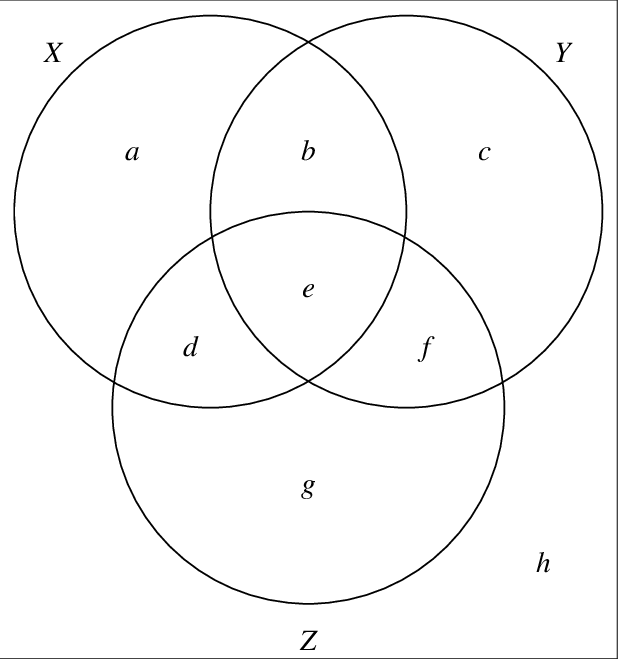
\includegraphics[scale=0.3]{img/Venn-diagram-visualization-of-a-3-event-probability-space-O.png}
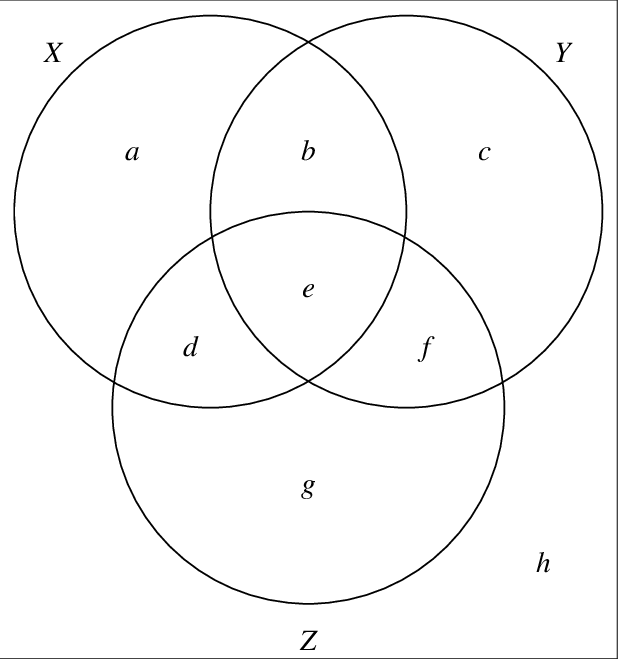
\includegraphics[scale=0.3]{img/Venn-diagram-visualization-of-a-3-event-probability-space-O.png}
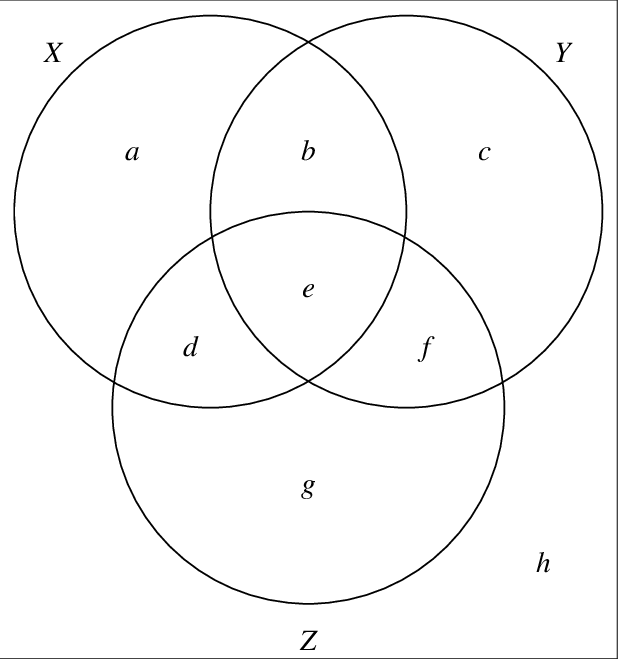
\includegraphics[scale=0.3]{img/Venn-diagram-visualization-of-a-3-event-probability-space-O.png}
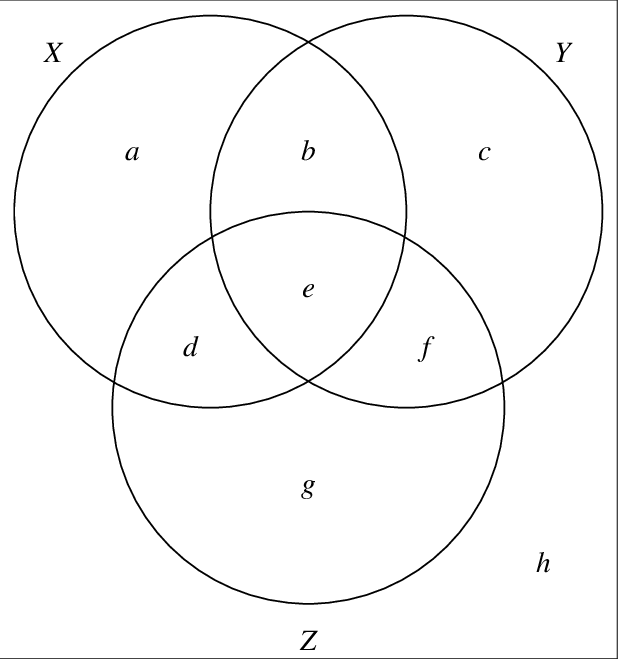
\includegraphics[scale=0.3]{img/Venn-diagram-visualization-of-a-3-event-probability-space-O.png}
\end{center}

\begin{defn}[Probabilidad\IS condicionada]
Sean $A,B$ sucesos de un suceso aleatorio. 

Se define la probabilidad condicionada $p(A/B)$ como la probablidad de que se produzca $A$ si sabemos que se ha producido $B$.

\[P(A/B) = \frac{P(A\cap B)}{P(B)}\]
\end{defn}

\textit{Este es un buen momento para hacer algún ejercicio. Página 349, ejer 36 por ejemplo. Recordamos que $P(A\cup B) = P(A) + P(B) - P(A\cap B)$}

\begin{defn}[Independencia de sucesos]
$A,B$ son sucesos independientes si y sólo si \[P(A/B) = P(A/\overline{B}) = P(A)\]
\end{defn}

\begin{theorem}
\[A,B \text{ independientes } \dimplies P(A\cap B) = P(A)·P(B)\]
\end{theorem}
\begin{proof}
\[\left.\begin{array}{c}
P(A/B) = \frac{P(A\cap B)}{P(B)} \dimplies P(A\cap B) = P(B)·P(A/B)\\A,B \text{ independientes } \dimplies P(A/B) = P(A)\end{array}\right\}*\]
\[(*) \implies P(A\cap B) = P(B)·\underset{P(A/B)}{P(A)} = P(B)·P(A)\]
\end{proof}

\begin{theorem}[Teorema\IS Probabilidad Total]
Sea $A_1,A_2,...,A_n$ un sistema completo de sucesos y sea $B$ otro suceso.
\[  
    P(B) = P(A_1\cap B) + P(A_2\cap B) + ... + P(A_n\cap B) = 
\]
\[
    P(B/A_1)·P(A_1) + P(B/A_2) · P(A_2) + ... + P(B/A_n)·P(A_n)
\]
\end{theorem}
\begin{theorem}[Teorema\IS de Bayes]
\[P(B/A) = \frac{P(A/B)·P(B)}{P(A)}\]
\end{theorem}
\begin{proof}
\[
\left.
\begin{array}{c}
    P(A\cap B) = P(A)·P(B/A)\\
    P(A\cap B) = P(B)·P(A/B)
\end{array}\right\} \implies P(A)·P(B/A) =  P(B)·P(A/B) \dimplies \]\[\dimplies P(B/A) = \frac{P(A/B)·P(B)}{P(A)} 
\]
\end{proof}


\paragraph{Bayesian trap (obtenido de youtube.com/Veritasium)}

\begin{example}
Se sabe que una enfermedad rara sólo afecta al 1\% de la población. 
%
El porcentaje de falsos positivos de las pruebas médicas es del 10\%, y el porcentaje de falsos negativos es del 1\%.

Intuitivamente, ¿cuál dirías que es la probabilida de tener la enfermedad sabiendo que has dado positivo en el test? ¿Podrías calcularlo numéricamente?

Los datos son: $P(E) = 0.01$, $P(-|E) = 0.01$ y $P(+|\overline{E})=0.1$

Aplicando el teorema de Bayes:

\[P(E|+) = \frac{P(+|E)·P(E)}{P(+)} = \frac{P(+|E)·P(E)}{P(+|E)·P(E) + P(+|\overline{E})·P(\overline{E})}= 0.01 \]
\end{example}


\section{Estadística}

A la hora de hacer un estudio estadístico buscamos obtener información sobre toda la población. A veces, esa cantidad de información es inmanejable e inconseguible. 
%
Por ejemplo, test de COVID a toda la población para ver cuántos lo han pasado, no es viable. 
%
Por ello, se selecciona una parte de la población y se le hacen los test a una parte para después extrapolar esos resultados.

Así, definimos:

\begin{defn}[Población]
\end{defn}

\begin{defn}[Muestra]
\end{defn}

\begin{defn}[Individuo]
\end{defn}

\textit{Nota: estos términos también se utilizan al tratar de tornillos en una fábrica.}

Este año vamos a trabajar y a distinguir los \concept[Parámetros\IS poblacionales]{parámetros poblacionales} de los \concept[Parámetros\IS muestrales]{muestrales}.
%
Llamaremos $\mu$ y $\sigma·$ a la media y desviación típica \emph{poblacionales} y $\bar{x}$ y $S$ a la media y desviación típica \emph{muestral}.

El \textbf{objetivo} de este tema es conseguir información sobre los parámetros poblacionales a partir de los parámetros muestrales. 

Para ello, antes de empezar es necesario que intentemos contestar la pregunta: ¿Cómo se asegura uno de que su muestra es buena? Porque si queremos saber lo que opinan los alumnos del colegio sobre la semipresencialidad y tomamos de muestra a los alumnos de 2º de Bachillerato, la información que saquemos no será fiable.

Necesitaremos que las muestras sean \concept[Representatividad de una muestra]{representativas} de toda la población, esto es, que refleje fielmente las características de la población.
%
Llamamos \concept{muestreo} al proceso por el que se construye una muestra de una población. 
%
Como seguro que te imaginas, hay distintos tipos de \textit{muestrear} una población. Vamos a verlos:

\subsection{Tipos de muestreo}

Los muestreos pueden ser aleatorios (si todos sus miembros tienen la misma posibilidad de ser elegidos) o no aleatorios (si no es así).
%
Dado que los muestreos aleatorios otorgan una mayor representatividad, nos centraremos en ellos:

Consideremos que eres el encargado de calidad de una fábrica de tornillos, que fabrica tornillos de distintos tipos.

\begin{itemize}
    \item Aleatorio simple.
        \subitem ¿Cuántas muestras se pueden formar?
        \subitem Estimación de los parámetros poblacionales desde los muestrales.
        \subitem Con reposición (días de la semana que se tienen que elegir), sin reposición (personas).
    \item Sistemático.
    \subitem Ordenados, de h en h (\concept{Constante de elevación}).
    \item Estratificado:
    \subitem Agrupación por característica. Estratos diferentes entre ellos. Elementos iguales en cada estrato.
    \subitem Afijación igual o proporcional.
    \subitem Dentro de cada estrato... ¿Aleatorio simple? ¿Sistemático?
    \item Conglomerados:
    \subitem División de cada característica. Conglomerados iguales entre ellos. Elementos diferentes en cada estrato.
    \subitem Dentro de cada estrato... ¿Aleatorio simple? ¿Sistemático?
\end{itemize}


\textbf{Importancia de los grupos control}

\section{Distribuciones de probabilidad}

Repaso de la distribución normal desde el PPT del departamento.
% 
\section{Inferencia estadística}

Inferir significa deducir algo o sacarlo como conclusión de otra cosa. \footnote{\href{https://dle.rae.es/inferir}{https://dle.rae.es/inferir}}

La tarea que nos va a mantener ocupados unas semanas va a ser la siguiente: \textit{Disponemos de una población con un parámetro desconocido. Tomaremos una muestra e inferiremos acerca del valor del parámetro poblacional utilizando información sobre la muestra.}


\subsection{Inferencia sobre la media}

Trabajaremos haciendo inferencia de la media. 
%
Tendremos poblaciones de las que conocemos su desviación típica (irreal en la vida diaria, pero así es el mundo de 2º de Bachillerato). Más adelante, en vuestra historia con las matemáticas, haréis inferencia de una manera más seria.

\begin{example}
Los de casa, rellenad en el enlace que os doy vuestro dato sobre la altura. Nuestra población serán todos los alumnos que están en casa. 

Una vez dispongamos de los datos, vamos a tomar una muestra para estimarla media de la población. ¿De cuánto cogemos la muestra? De cuantas más personas, mejor, ¿no?

 Hay un resultado fundamental en inferencia estadística (Teorema Central del Límite) del que se deduce que la \concept[Distribución de la media muestral]{media muestral se distribuye} $\overline{X} \sim N\left(\mu,\frac{\sigma}{\sqrt{n}}\right)$
\end{example}

\begin{example}
Ejemplo de cálculo, siguiendo el libro.
\end{example}

\subsubsection{Estimación de la media}
Lo que acabamos de hacer no es inferir, sino entender que la media muestral se distribuye según una distribución normal cuando tenemos suficientes datos (>30) o los datos poblacionales siguen una distribución normal. 

¿Qué ocurre si desconocemos la media de la población y queremos inferirla con una muestra?
%
Tenemos \textbf{dos opciones}, estimación puntual y estimación por intervalos.

\subparagraph{Estimación puntual: } Inferimos $\mu$ a partir de $\overline{X}$ y decimos: $\mu \sim \overline{X}$

\subparagraph{Estimación por intervalos de confianza: } Inferimos $\mu$ a partir de $\overline{X}$ y $\sigma$ y decimos: $\overline{X} - E < \mu < \overline{X} + E$, donde $E$ es una amplitud del intervalo que dependerá de varios factores:
\begin{itemize}
    \item \textbf{La confianza:} no hay ninguna duda que $-\infty<x<\infty$. Esta inferencia tiene una confianza del 100\%, pero no da mucha información. 
    \item \textbf{La desviación típica poblacional $\sigma$:} ya que, cuanto más dispersos estén los datos de la población, más variabilidad tendrá $\overline{X}$ y más grande deberá ser el intervalo para la misma confianza.
\end{itemize}

\begin{theorem}[Intervalo de confianza para la media]

Un intervalo de confianza para la media población de una distribución normal con desviación típica conocida, con un nivel de confianza $1-\alpha$ construido a partir de una muestra de tamaño $n$ es:
\[\left(\overline{x} - \mathcal{E} , \overline{x} + \mathcal{E}\right)\]



Donde $\mathcal{E} = z_{\rfrac{\alpha}{2}}·\frac{\sigma}{\sqrt{n}}$ y se denomina \concept{Error máximo admisible} (no es otra cosa que la amplitud del intervalo de confianza).

Y $\zalfamedios$ es el valor que cumple:
\[ P(\left -\zalfamedios < Z < \zalfamedios\right) = 1-\alpha\]

\obs Nivel de confianza $1-\alpha$ $\dimplies$ Nivel de significación $\alpha$
\end{theorem}

\begin{example}
Ejemplo de cálculo sacado del libro.
\end{example}

\paragraph{Ejercicio 11}

\paragraph{Cálculo del tamaño de la muestra: } Dado que $\mathcal{E} = z_{\rfrac{\alpha}{2}}·\frac{\sigma}{\sqrt{n}}$, podríamos buscar qué tamaño de la muestra debo escoger para construir un intervalo de confianza de amplitud dada.

\begin{example}
Ejemplo de cálculo del libro.
\end{example}

\textbf{Ejercicio 16}

\subsection{Inferencia sobre la proporción}

Lo primero que necesitamos tener claro es lo que es una \concept{proporción}:


\newcommand{\matp}{\rho}
Llamaremos $\hat{P}$ a la distribución de la proporción meustral. Será $\matp$ el parámetro a estimar.

\[\hat{P} \sim N\left(\matp,\sqrt{\frac{\matp q}{n}}\right), q=1-\matp\]

\begin{example}
Ejemplo de cálculo del libro
\end{example}

\subsubsection{Estimación sobre la proporción}

Aquí también tenemos la estimación puntual $\left(\hat{P} \approx \matp\right)$ y una estimación por intervalos de confianza.


\begin{prop}[Intervalo de confianza para la proporción]

Un intervalo de confianza para la proporción de individuos que cumplen una característica en una población, con un nivel de confianza $1-\alpha$ construido a partir de una muestra de tamaño $n$ es:
\[\left(\hat{p} - \mathcal{E} , \hat{p} + \mathcal{E}\right)\]



Donde $\mathcal{E} = z_{\rfrac{\alpha}{2}}·\sqrt{\frac{\hat{p}\hat{q}}{n}}$ y se denomina \concept{Error máximo admisible} (no es otra cosa que la amplitud del intervalo de confianza).

Y $\zalfamedios$ es el valor que cumple:
\[ P(\left -\zalfamedios < Z < \zalfamedios\right) = 1-\alpha\]

\obs Nivel de confianza $1-\alpha$ $\dimplies$ Nivel de significación $\alpha$
\end{prop}

\begin{example}
Ejemplo de cálculo del libro
\end{example}

\textbf{Ejercicio 17}

\paragraph{Cálculo del tamaño de la muestra: } Dado que $\mathcal{E} = z_{\rfrac{\alpha}{2}}·\sqrt{\frac{\hat{p}\hat{q}}{n}}$, podríamos buscar qué tamaño de la muestra debo escoger para construir un intervalo de confianza de amplitud dada.

\begin{example}
Ejemplo de cálculo del libro.
\end{example}

\textbf{Ejercicio 19}
%
\section{Estadística unidimensional descriptiva}

\paragraph{¿Para qué sirve la estadística?} Sirve para hacer predicciones. Estudiar los datos permite obtener información para poder hacer predicciones. 

Por ejemplo, si la nota media en una clase es de $\overline{x}=5$ y sabemos que los datos varían muy poco, es probable que si he perdido un examen, su nota fuera a ser un 5. En cambio, si la nota media es $\overline{x} = 5$ pero los datos están muy dispersos y hay desde $0$ hasta $10$, no tengo mucha posibilidad de estimar su nota sin equivocarme.

\subsection{Vocabulario estadístico}

Rellenar de ejemplos el margen del libro a lápiz.

\begin{itemize}
	\item Población
	\item Muestra
	\item Individuo
	\item Variables:
		\subitem Cualitativas o cuantitativas.
		\subitem Discretas o continuas.
\end{itemize}

\subsection{Tabla de frecuencias}
Ejercicio 4.

\subsection{Medidas}

\subsubsection{Centralización}
Ejercicios 10 y 12.

\subsubsection{Posición}

\subsubsection{Dispersión}

\section{Probabilidad, binomial y normal}

\subsection{Probabilidad}

\subsection{Binomial}

\subsection{Normal}


\section{Estadística bidimensional}


%Fin 3ª evaluación


\printindex
\end{document}
\grid
